\usepackage[utf8x]{inputenc}
\usepackage[T1]{fontenc}
\usepackage{libertine}
\usepackage[spanish]{babel}
\spanishdatedel
\usepackage[pdftex]{graphicx}
\usepackage[usenames,dvipsnames,x11names,table,svgnames]{xcolor}
\usepackage[colorlinks=true,urlcolor=blue,linkcolor=black,anchorcolor=black,citecolor=black]{hyperref}
\usepackage{mathtools,amssymb,amsfonts,amsmath,amsthm,mathrsfs,bm,times,mathabx}
\usepackage[makeroom]{cancel}
\usepackage{multicol}
\usepackage{geometry}
\usepackage{background}
\usepackage{caption,subcaption}
\usepackage{enumitem}
%\geometry{
%	tmargin=1cm, 
%	bmargin=0.5cm, 
%	lmargin=0.5cm, 
%	rmargin=1cm,
%	headheight=1.5cm,
%	headsep=0.8cm,
%	footskip=0.5cm}
\hypersetup{pdfinfo={
		Title={Apuntes de clases de Teoría de números},
		Author={Jimmy Espinoza Palacios},
		Keywords={Divisibilidad, Congruencias, Funciones aritméticas},
		Subject={Teoría de números},
		Producer={TeXstudio 2.12.6},
		Creator={pdfTeX Version 3.14159265-2.6-1.40.18 TeX Live 2018 Debian}
}}

\backgroundsetup{%
	scale=1,       %% change accordingly
	angle=0,       %% change accordingly
	opacity=.1,    %% change accordingly
	contents={\begin{tikzpicture}[remember picture,overlay]
		\node at ([yshift=11pt,xshift=5pt]current page.center) {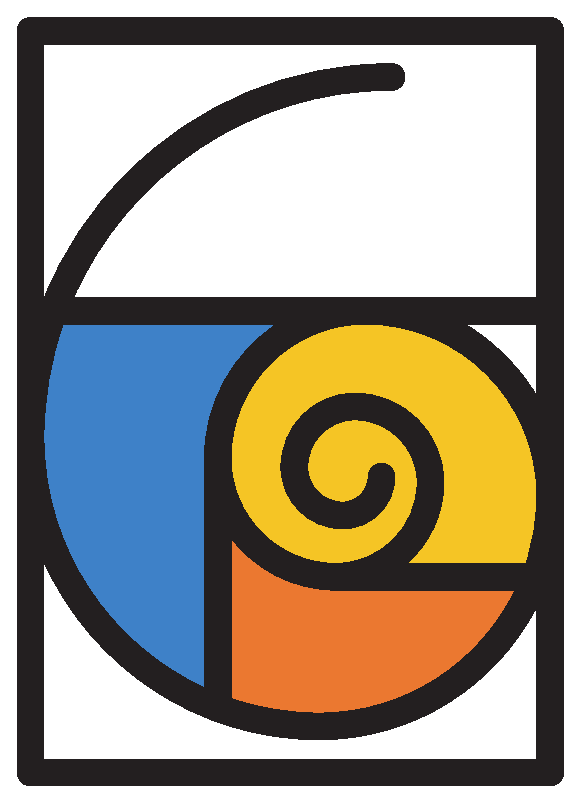
\includegraphics[width=8.1cm]{gemtransparente}};    %% yshift and xshift for example only
		\end{tikzpicture}}
}

\newcommand*{\colorboxed}{}
\def\colorboxed#1#{%
	\colorboxedAux{#1}%
}
\newcommand*{\colorboxedAux}[3]{%
	% #1: optional argument for color model
	% #2: color specification
	% #3: formula
	\begingroup
	\colorlet{cb@saved}{.}%
	\color#1{#2}%
	\boxed{%
		\color{cb@saved}%
		#3%
	}%
	\endgroup
}

%\usepackage[citestyle=numeric,style=numeric,backend=biber]{biblatex}
%\addbibresource{num.bib}
\DeclareMathOperator{\mcd}{mcd}
\newcommand{\MVAt}{{\usefont{U}{mvs}{m}{n}\symbol{`@}}} % Se prefiere no usar el paquete marvosym cuando esté cargada mathabx.
\renewcommand{\qedsymbol}{$\blacksquare$}
\newtheorem{definition}{Definición}[chapter] %chapter, section
\newtheorem{theorem}{Teorema}[chapter] %chapter section
\newtheorem{remark}{Observación}[chapter]
\theoremstyle{definition}
\pagestyle{empty}